% !TEX root = ./paper.tex

\section{Evaluation}
In this section, we experimentally evaluate our technique for learning graph-based heuristics.
We aim to answer the following research questions:

\begin{itemize}
\item {\bf Effectiveness and Generality:}
How effectively does the learned heuristic perform compared to the state-of-the-art heuristics?
Is it generally applicable for different analysis tasks without manual effort for designing application-specific features?

\item {\bf Learning Algorithm:}
How much does the learning cost?
How does the hyper-parameter $\hyper$ affect the performance of the learned heuristics?

% i.e.,
%~\Scaler~\cite{Li2018b},~\Zipper~\cite{Li2018a},~\Data~\cite{JeJeChOh17},~\Mahjong~\cite{Tan2017}?
\item {\bf Learned Insight:}
Does our approach produce explainable heuristics?
What are the insights learned from the generated heuristics?
\end{itemize}

\myparagraph{Overall Setting}
We implemented our approach, as a tool \OurCtx, on top of \Doop~\cite{BravenboerS09},
a pointer analysis framework for Java that has been widely used in prior works
~\cite{Smaragdakis2014,JeJeChOh17,JeJeOh18,Tan2017,TanLX16}.
%In particular, we applied our approach to learn heap abstraction and context-sensitivity heuristics from FPG and OAG, respectively.
%We implemented our technique on the two different artifacts~\cite{Tan2017,Li2018b}, the state-of-the-art context-sensitivity and heap abstraction heuristics, to demonstrate the effectiveness of our learned heuristics on both heuristics.
For the precision and scalability metrics, we follow existing works~\cite{Tan2017,Li2018a,Li2018b,JeJeChOh17} and use the number of may-fail casts alarms and the time spent on each analysis.
We also use the number of polymorphic call sites (i.e. call sites whose targets are not uniquely determined by each pointer analysis) and call-graph edges as additional precision metrics. For all precision metrics, the lower is the better.
%Polymorphic call sites present call sites that are not disambiguated into monomorphic calls.
We set the time budget as 3 hours (10,800 sec) for all analyses.
For the hyper-parameter $\hyper$, we chose the one among various values (e.g., 0.1, 0.2, ..., 0.9) via cross validation (we explain how this is done in section~\ref{sec:learning_alg}).
For each feature, we limit it to have at most three nodes due to scalability.
All the experiments were done on a machine with i7 CPU and 64 GB RAM running Ubuntu 16.04 (64bit).
We used the OpenJDK (1.6.0\_24) library.


%\myparagraph{Benchmarks}
We used a total of 17 programs: 10 programs (luindex, lusearch, antlr, pmd$_{m}$, chart, eclipse, fop, bloat, xalan, and jython) from the DaCapo 2006-10-MR2 benchmark suite~\cite{Blackburn2006}
and 7 programs (pmd$_{s}$, jedit, briss, soot, findbugs, JPC, and checkstyle) obtained from the artifacts provided by~\cite{Tan2017} and~\cite{Li2018b}.
%Here, we used two different versions of pmd where pmd$_{m}$ is a program in Dacapo benchmarks used in~\cite{Tan2017}, and pmd$_{s}$ is an open-source application used in~\cite{Li2018b}.
Here, we used two different versions of pmd where pmd$_{m}$ is a small program used by~\cite{Tan2017}, and pmd$_{s}$ is an open-source application used by~\cite{Li2018b}.
We split the benchmark programs into training, validation, and test sets.
The training and validation sets are used for learning a heuristic, and the test set is used for evaluating the performance of the learned heuristic.
For the training set, we used relatively small benchmarks, because our algorithm includes a process
to obtain minimal abstractions and this task is too expensive to run for large programs.
The validation set is used for choosing the hyper-parameter $\hyper$; we chose the one that leads the heuristic to the best performance on the validation set.
%After training heuristics with various values of $\hyper$, we chose the one which shows the best performance on a validation program {\tt findbugs}.
%We discuss the importance of the value of $\hyper$ later in detail.


\subsection{Effectiveness and Generality}
We demonstrate the effectiveness and generality of our technique by comparing it with two state-of-the-art graph-based heuristics: \Scaler~\cite{Li2018b} and \Mahjong~\cite{Tan2017}.

%comparing the performance of the generated heuristics to existing context-sensitivity heuristics and heap abstraction heuristics.

\subsubsection{Comparison with Scaler}\label{sec:comparescaler}
%\textcolor{black}{
\myparagraph{Setting}
\Scaler~is a context-sensitivity heuristic that works on the object allocation graph (OAG)~\cite{Li2018b}. From the OAG, it infers a policy to assign one of 2-object-sensitivity, 2-type-sensitivity, 1-type-sensitivity, and context-insensitivity to each method.
We used the same pre-analysis of \Scaler~to obtain the OAG and let our technique produce a heuristic.
We set $\CallDepth$ in Section~\ref{sec:param-context} to 3, where 0, 1, 2, and 3 correspond to context-insensitivity, 1-type-sensitivity, 2-type-sensitivity, and 2-object-sensitivity, respectively.
Unlike \Scaler, our heuristic assigns a context for each heap allocation site.
It poses $4^N$ possibilities where $N$ denotes the number of allocation-sites in the program.
%}
%as Scaler does.}
% that assigns one of the four context-sensitivity options to each method call.
%To compare with existing context-sensitivity heuristics, we learned such heuristics using the object-allocation-graphs (OAG) on which the state-of-the-art context-sensitivity heuristic \Scaler~was developed.
%For fair comparison, our learned heuristic,~\OurCtx, assigns either 2-object-sensitivity, 2-type-sensitivity, 1-type-sensitivity, or context-insensitive analysis to each method call as \Scaler~does.
%We also apply 2-object-sensitivity if receiver objects have a type \emph{java.util.*}, like \Scaler~does to preserve the precision.
%In our framework, since we explained that object-sensitivity heuristics assign different depth (e.g., 0,1, or 2) of context to each method call, these four analysis heuristics correspond to 3, 2, 1, and 0, respectively.
%This abstraction still satisfies the monotonicity as 2-object-sensitivity is strictly more precise than 2-type-sensitivity~\cite{Smaragdakis2011}.

Although the primary  objective in this evaluation is to compare with \Scaler, we evaluated two more heuristics as well: \Zipper~\cite{Li2018a} and \Data~\cite{JeJeChOh17}.
\Zipper~is another graph-based context-sensitivity heuristic that works on the precision flow graph (PFG).
\Data~is not graph-based, but we include it because \Data~is currently the state-of-the-art data-driven pointer analysis algorithm (with hand-crafted features).
%n object-sensitivity heuristic from machine learning technique with hand crafted features~\cite{JeJeChOh17}.
%the three graph-based heuristics \OurCtx,\Scaler, and \Zipper~use context-insensitive analysis as a pre-analysis to obtain a graph.
%Meanwhile, \Data~is another object-sensitivity heuristic from machine learning technique with hand crafted features~\cite{JeJeChOh17}.
In short, we compare the following pointer analysis algorithms: %to demonstrate the effectiveness of our learned context-sensitivity heuristic:

\begin{itemize}
\item \Scaler: A hand-crafted graph-based object-sensitivity heuristic for OAG~\cite{Li2018b}
\item \OurCtx: Our learning-based graph-based object-sensitivity heuristic for OAG
\item \Zipper: A hand-crafted graph-based object-sensitivity heuristic for PFG~\cite{Li2018a}
\item \Data: A state-of-the-art learning-based object-sensitivity heuristic~\cite{JeJeChOh17}
\item \twoobjH: The 2-object-sensitivity with 1-context-sensitive heap (precision upper bound)
\item \Insens: The context-insensitive analysis (scalability upper bound)
\end{itemize}
%  All heuristics use allocation-site-based heap abstraction.
%Our framework generated 195 features in total as an object-sensitivity heuristic (e.g., 68 features for 2-object-sensitivity, 28 for 2-type-sensitivity, and 99 features for 1-type-sensitivity).
%The learning procedure takes about 220 hours in total, where 168 hours are for getting minimal abstractions over the training programs
%and 52 hours for generating the features.


%To compare~\OurCtx~with~\Scaler,
We used three programs (luindex, lusearch, antlr) as the training set, one program (findbugs) as the validation set,
and the remaining thirteen programs (pmd$_{s}$, chart, eclipse, jedit, briss, soot, jython, pmd$_{m}$, fop, bloat, JPC, checkstyle, xalan) as the test set.
We chose findbugs as a validation program because it is a popular Java application and
requires suitable heuristics to be analyzed cost-effectively.
For example, \twoobjH~does not terminate on this program even after thousands of seconds or more.


\myparagraph{Results}
\begin{table}[]
\setlength\extrarowheight{-1pt}
\caption{Performance of the context-sensitivity heuristics against benchmarks.
%For all metrics, the lower is the better.
%For precision metric, we use the number of may-fail casts(\#may-fail casts) and polymorphic call sites (\#poly-call sites) whose targets are not uniquely determined by each pointer analysis.
%For scalability metric, we use analysis time, and the number in a parenthesis presents the sum of time spent during pre-analysis process.
%\#call-graph-edges for the training and validation programs are omitted due
%    to the lack of space.
}
\label{tbl:contextAbstraction}
\scriptsize
\begin{tabular}{@{}r|clrrrrrr@{}}
\toprule
\multicolumn{1}{c}{}               &                           & \multicolumn{1}{c}{} & \multicolumn{1}{c}{\OurCtx} & \multicolumn{1}{c}{\Scaler} & \multicolumn{1}{c}{\Zipper} & \multicolumn{1}{c}{\Data} & \multicolumn{1}{c}{\twoobjH} & \multicolumn{1}{c}{\Insens} \\ \midrule
\multirow{9}{*}{\rotatebox[origin=c]{90}{Training programs}} & \multirow{3}{*}{luindex}  & analysis time (s)    & 22(+22)                       & 36(+17)                         & 33(+17)                         & 19                         & 36                       & 15                         \\
                                   &                           & \#may-fail casts     & 297                      & 297                        & 310                        & 341                         & 297                      & 734                        \\
                                   &                           & \#poly-call sites    & 682                      & 675                        & 677                        & 702                         & 675                         & 940                        \\
                                   %&                           & \#call-graph-edges   & 29,045                   & 29,021                     & 29,025                     & 29,196                         & 29,021                         & 33,130                      \\
\cmidrule(){2-9}
                                   & \multirow{3}{*}{lusearch} & analysis time (s)    & 24(+21)                       & 63(+15)                         & 62(+17)                         & 19                         & 66                       & 15                         \\
                                   &                           & \#may-fail casts     & 299                      & 299                        & 305                        &  347                        & 299                      & 844                        \\
                                   &                           & \#poly-call sites    & 858                      & 850                        & 853                        & 883                         & 850                         & 1,133                      \\
                                   %&                           & \#call-graph-edges   & 31,838                   & 31,811                     & 31,817                     & 31,995                         & 31,811                         & 36,343                      \\
\cmidrule(){2-9}
                                   & \multirow{3}{*}{antlr}    & analysis time (s)    & 50(+94)                       & 51(+24)                         & 84(+26)                           & 33                         & 109                      & 24                         \\
                                   &                           & \#may-fail casts     & 409                      & 412                        & 420                           & 513                         & 409                      & 918                        \\
                                   &                          & \#poly-call sites    & 1,495                    & 1,488                      & 1,488                           & 1,517                         & 1,487                         & 1,729                      \\
                                   %&                           & \#call-graph-edges   & 47,273                   & 49,398                     & 47,233                           & 47,358                         & 47,232                         & 50,652                      \\
\midrule \midrule
\multirow{28}{*}{\rotatebox[origin=c]{90}{Test programs}} & \multirow{4}{*}{pmd$_{s}$}      & analysis time (s)    & 710(+92)                      & 494(+49)                        &  $>$10,800                          & 117                         & $>$10,800     & 48                         \\
                                   &                           & \#may-fail casts     & 2,075                    & 2,176                      & -                           & 2,145                         & -                         & 2,948                      \\
                                   &                           & \#poly-call sites    & 3,507                    & 3,536                      & -                           & 3,647                         & -                         & 4,183                      \\
                                   &                           & \#call-graph-edges   & 92,589                   & 92,775                     & -                           & 94,328                         & -                         & 104,457                     \\\cmidrule(){2-9}

                                   & \multirow{4}{*}{chart}    & analysis time (s)    & 63(+73)                       & 184(+48)                        & 113(+56)                        & 35                         & 196                      & 48                       \\
                                   &                           & \#may-fail casts     & 998                      & 976                        & 888                        & 974                         & 883                      & 1,810                         \\
                                   &                           & \#poly-call sites    & 1,392                    & 1,402                      & 1,379                      & 1,435                         & 1,378                         & 1,852                      \\
                                   &                           & \#call-graph-edges   & 52,544                   & 53,198                     & 52,377                     & 52,647                         & 52,374                         & 63,453                     \\\cmidrule(){2-9}
                                   & \multirow{4}{*}{eclipse}  & analysis time (s)    & 1,395(+103)                    & 652(+92)                        & 9,701(+114)                           & 159                         & $>$10,800     & 91                         \\
                                   &                           & \#may-fail casts     & 2,989                    & 3,211                      & 2,897                           & 3,178                         & -                         & 4,190                      \\
                                   &                           & \#poly-call sites    & 8,418                    & 8,486                      & 8,390                           & 8,627                         & -                         & 9,197                      \\
                                   &                           & \#call-graph-edges   & 144,873                  & 145,953                    & 143,727                           & 146,512                         & -                         & 161,222                     \\\cmidrule(){2-9}
                                   & \multirow{4}{*}{jedit}    & analysis time (s)    & 845(+90)                      & 1,377(+79)                      &   $>$10,800                         & 137                         & $>$10,800      & 78                         \\
                                   &                           & \#may-fail casts     & 2,196                    & 2,397                      &  -                          & 2,298                         &  -                        & 3,398                      \\
                                   &                           & \#poly-call sites    & 3,917                    & 4,012                      &  -                          & 4,091                         &  -                        & 4,769                      \\
                                   &                           & \#call-graph-edges   & 98,401                   & 99,536                     &  -                          & 99,697                         &  -                        & 120,309                     \\\cmidrule(){2-9}
                                   & \multirow{4}{*}{briss}    & analysis time (s)    & 2,368(+169)                    & 907(+151)                           & $>$10,800                           & 499                         & $>$10,800     & 149                        \\
                                   &                           & \#may-fail casts     & 3,065                    & 3,428                      &  -                          & 3,162                         &  -                        & 4,904                      \\
                                   &                           & \#poly-call sites    & 5,099                    & 5,323                      &  -                          & 5,291                         &  -                        & 6,297                      \\
                                   &                           & \#call-graph-edges   & 150,351                  & 152,761                    &  -                          & 151,861                         &  -                        & 176,785                     \\\cmidrule(){2-9}
                                   & \multirow{4}{*}{soot}     & analysis time (s)    & $>$10,800     & 883(+727)                        & $>$10,800                           & $>$10,800                         & $>$10,800     & 698                        \\
                                   &                           & \#may-fail casts     &  -                        & 10,549                     &   -                         & -                         &   -                       & 16,570                     \\
                                   &                           & \#poly-call sites    &  -                        & 14,822                     &   -                         & -                         &   -                       & 16,532                     \\
                                   &                           & \#call-graph-edges   &  -                        & 374,877                    &  -                          & -                         &  -                        & 415,476                     \\\cmidrule(){2-9}
                                   & \multirow{4}{*}{jython}   & analysis time (s)    & $>$10,800     & 314(+96)                        & $>$10,800                           & 425                         & $>$10,800     & 73                         \\
                                   &                           & \#may-fail casts     & -                         & 1,852                      &  -                          & 1,773                          &  -                        & 2,234                      \\
                                   &                           & \#poly-call sites    & -                         & 2,500                      &  -                          & 2,481                         & -                         & 2,778                      \\
                                   &                           & \#call-graph-edges   &  -                        & 107,410                     & -                           & 106,837                         &  -                        & 114,856
\\\midrule \midrule
\multirow{3}{*}{\rotatebox[origin=c]{90}{Valid}}
                                   & \multirow{3}{*}{findbugs} & analysis time (s)    & 305(+58)                      & 191(+36)                        & 1,399(+43)                           & 59                         & 2,458                    & 35                      \\
                                   &                           & \#may-fail casts     & 1,436                    & 1,452                      & 1,412                           & 1,663                         & 1,409                    & 2,508                         \\
                                   &                           & \#poly-call sites    & 2,188                    & 2,195                      & 2,182                           & 2,220                         & 2,182                         & 2,925                      \\
                                   %&                           & \#call-graph-edges   & 65,874                   & 66,177                     &  65,838                          & 66,028                         &  65,836                        & 77,370                     \\
\bottomrule
\end{tabular}
\end{table} 

% Please add the following required packages to your document preamble:
% \usepackage{booktabs}
% \usepackage{multirow}
\begin{table}[]
\setlength\extrarowheight{-1pt}
\caption{Performance comparison among various context sensitivity heuristics against the left six benchmarks. All the notations are the same with Table~\ref{tbl:contextAbstraction}.}
\label{appendix:ctx}
\centering
\footnotesize
\begin{tabular}{@{}c|clrrrrrr@{}}
\toprule
\multicolumn{1}{c}{}&\multicolumn{1}{c}{}        & \multicolumn{1}{c}{} & \multicolumn{1}{c}{\OurCtx} & \multicolumn{1}{c}{\Scaler} & \multicolumn{1}{c}{\Zipper} & \multicolumn{1}{c}{\Data} & \multicolumn{1}{c}{\twoobjH} & \multicolumn{1}{c}{\Insens} \\ \midrule
\multirow{28}{*}{\rotatebox[origin=c]{90}{Test programs}}&\multirow{4}{*}{pmd$_m$}       & analysis time (s)    & 43(+67)                      & 55(+44)                    & 57(+78)                    & 30                       & 67                       & 23                         \\
&                            & \#may-fail casts     & 288                          & 287                        & 300                        & 327                      & 287                      & 679                        \\
&                            & \#poly-call sites    & 643                          & 636                        & 638                        & 667                      & 636                      & 885                        \\%\cmidrule(){2-9}
&                            & \#call-graph-edges   & 27,074                        & 27,052                      & 27,056                      & 27,147                    & 27,052                    & 30,328                      \\\cmidrule(){2-9}
&\multirow{4}{*}{fop}        & analysis time (s)    & 212(+88)                     & 341(+54)                   & 533(+71)                   & 74                       & 949                      & 53                         \\
&                            & \#may-fail casts     & 1,568                         & 1,732                       & 1,449                       & 1,600                     & 1,446                     & 2,458                       \\
&                            & \#poly-call sites    & 2,876                         & 2,945                       & 2,848                       & 3,009                     & 2,844                     & 3,585                       \\%\cmidrule(){2-9}
&                            & \#call-graph-edges   & 71,612                        & 72,556                      & 71,418                      & 72,113                    & 71,408                    & 84,330                      \\\cmidrule(){2-9}
&\multirow{4}{*}{bloat}      & analysis time (s)    & 216(+30)                     & 290(+21)                   & 2402(+23)                  & 44                       & 2,422                     & 20                         \\
&                            & \#may-fail casts     & 1,215                         & 1,222                       & 1,205                       & 1,288                     & 1,193                     & 1,924                       \\
&                            & \#poly-call sites    & 1,458                         & 1,465                       & 1,429                       & 1,496                     & 1,427                     & 2,014                       \\%\cmidrule(){2-9}
&                            & \#call-graph-edges   & 53,641                        & 53,867                      & 53,147                      & 54,059                    & 53,143                    & 61,150                      \\\cmidrule(){2-9}
&\multirow{4}{*}{JPC}        & analysis time (s)    & 118(+69)                     & 274(+38)                   & 266(+55)                   & 45                       & 398                      & 37                         \\
&                            & \#may-fail casts     & 1,427                         & 1,552                       & 1,343                       & 1,472                     & 1,345                     & 2,261                       \\
&                            & \#poly-call sites    & 4,210                         & 4,228                       & 4,187                       & 4,322                     & 4,186                     & 4,924                       \\%\cmidrule(){2-9}
&                            & \#call-graph-edges   & 79,912                        & 80,098                      & 79,787                      & 80,208                    & 79,783                    & 94,569                      \\\cmidrule(){2-9}
&\multirow{4}{*}{checkstyle} & analysis time (s)    & 133(+70)                     & 264(+45)                   & 396(+52)                   & 69                       & 1,693                     & 44                         \\
&                            & \#may-fail casts     & 600                          & 625                        & 590                        & 644                      & 581                      & 1,114                       \\
&                            & \#poly-call sites    & 1,052                         & 1,038                       & 1,040                       & 1,089                     & 1,035                     & 1,444                       \\%\cmidrule(){2-9}
&                            & \#call-graph-edges   & 9,516                         & 9,514                       & 48,830                      & 48,996                    & 48,809                    & 57,490                      \\\cmidrule(){2-9}
&\multirow{4}{*}{xalan}      & analysis time (s)    & 226(+64)                     & 539(+38)                   & 119(+45)                   & 44                       & 881                      & 37                         \\
&                            & \#may-fail casts     & 567                          & 579                        & 556                        & 604                      & 533                      & 1,182                       \\
&                            & \#poly-call sites    & 1,533                         & 1,523                       & 1,533                       & 1,583                     & 1,522                     & 1,898                       \\%\bottomrule
&                            & \#call-graph-edges   & 45,269                        & 44,887                      & 9,125                       & 45,549                    & 44,871                    & 5,1302                      \\ \bottomrule 
\end{tabular}
\end{table}


%\myparagraph{Result of context-sensitivity heuristic}
Table~\ref{tbl:contextAbstraction} and~\ref{appendix:ctx} present the performance of the context-sensitivity heuristics described above.
The number in a parenthesis for graph-based heuristics (i.e. \OurCtx, \Zipper, and \Scaler)
represents the sum of time spent on performing the pre-analysis (i.e. context-insensitive analysis) and running the heuristics on the graphs for extracting context abstractions.

The results show that our technique can automatically generate a cost-effective heuristic that performs as competitive as the state-of-the-art object-sensitivity heuristics.
%In comparison to the baseline heuristic~\Scaler, which employs the same graph OAG, \OurCtx~consistently shows a better precision than \Scaler~
%with some losses in scalability.
Compared to the baseline heuristic~\Scaler, which employs the same graph OAG, \OurCtx~%consistently
shows a better precision than \Scaler~
with some losses in scalability for the test programs pmd$_{s}$, eclipse, and briss.
For example, \OurCtx~reports 101 less may-fail casts alarms than \Scaler~ for the test program pmd$_{s}$
while taking 216 more seconds.
In addition, \OurCtx~shows better performance in both precision and scalability than \Scaler~on the test programs (except pmd$_m$) in Table~\ref{appendix:ctx}.
For example, in jedit, \OurCtx~produces 201 less alarms with 35\% less analysis time.
In comparison to \Zipper, \OurCtx~consistently outperforms in scalability.
For example, \OurCtx~successfully analyzed pmd$_{s}$, jedit, and briss with remarkably less costs when \Zipper~fails to analyze them within the time budget.
In comparison to \Data, the result shows that \OurCtx~performs far better in precision.
%Although \Data~presents better scalability than \OurCtx, it produces about 100$\sim$300 \TODO{concrete numbers} more alarms for the testing programs.
Although \Data~presents better scalability than \OurCtx, it produces more than 92 alarms for the test programs pmd$_{s}$, eclipse, jedit and briss.
Compared to \twoobjH, \OurCtx~ shows better performance in scalability for the majority of test programs which \twoobjH~fails to analyze within the given time budget (3 hours).

\subsubsection{Comparison with Mahjong}\label{sec:eval_heap}
\myparagraph{Setting}
%To show the generality of our framework,
%we additionally evaluated our technique to learn a graph-based heap abstraction heuristic from field points-to graph (FPG) which the state-of-the-art heap abstraction heuristic \Mahjong~uses.

\Mahjong~is a graph-based heap abstraction heuristic that works on the field points-to graph (FPG)~\cite{Tan2017}.
From the FPG, which is obtained by running a context-insensitive pre-analysis, \Mahjong~infers a policy that determines whether to merge objects allocated in different allocation sites.
We used the same pre-analysis to obtain the FPG and let our technique produce a heap abstraction heuristic.
Unlike \Mahjong, our heap abstraction heuristic (i.e. \OurHeap) assigns `{\it type}' (type-based heap abstraction) or `{\it alloc}' (allocation-site-based heap abstraction) to each heap allocation-site which poses
$2^N$ possibilities where $N$ denotes the number of allocation-sites in the program.
%\todored{needs more explanation how $2^\mbh$ possibilities are selected...}
We compare the following four analyses:
\begin{itemize}
\item \Mahjong: The state-of-the-art graph-based heap abstraction heuristic~\cite{Tan2017}
\item \OurHeap: Our learning-based graph-based heap abstraction heuristic
\item \AllocBased: The uniform allocation-site-based heap abstraction (precision upper bound)
\item \TypeBased: The uniform type-based heap abstraction (scalability upper bound)
\end{itemize}
Following \Mahjong~\cite{Tan2017}, all analyses above use 3-object-sensitivity with 2-context-sensitive heap.

For this evaluation, we used the same benchmark programs in the section~\ref{sec:comparescaler}.
We used four programs (luindex, lusearch, antlr, pmd$_{m}$) as the training set and
twelve programs (fop, chart, bloat, xalan, JPC, checkstype, eclipse, pmd$_{s}$, jecit, briss, soot, jython) as the test set.
We also used findbugs as a validation program.
% as we did for the comparison with~\Scaler
%From the 17 benchmarks, we used four programs (luindex, lusearch, antlr, pmd$_{m}$) as the training set.


\begin{table}[]
\setlength\extrarowheight{-1.5pt}
\caption{Performance of the heap abstraction heuristics against benchmarks.
The notions are the same with those in Table~\ref{tbl:contextAbstraction}.}
\label{tbl:heapAbstraction}
\centering
\scriptsize
\begin{tabular}{@{}c|clrrrr@{}}
\toprule
\multicolumn{1}{c}{}                                    &                             &                    & \multicolumn{1}{c}{\OurHeap} & \multicolumn{1}{c}{\Mahjong} & \multicolumn{1}{c}{\AllocBased} & \multicolumn{1}{c}{\TypeBased} \\ \midrule
\multirow{16}{*}{\rotatebox[origin=c]{90}{Training programs}} & \multirow{4}{*}{luindex}    & analysis time(s)   & 23(+90)                       & 42(+21)                          & 5,475                           & 19                             \\
                                   &                             & \#may-fail casts   & 358                      & 358                         & 358                             & 795                            \\
                                   &                             & \#poly-call sites  & 928                      & 918                         & 915                             & 1,128                          \\
                                   &                             & \#call-graph-edges & 33,450                   & 33,365                      & 33,356                          & 37,898                         \\ \cmidrule(l){2-7}
                                   & \multirow{4}{*}{lusearch}   & analysis time(s)   & 21(+92)                       & 43(+19)                          & \textgreater{}10,800            & 19                             \\
                                   &                             & \#may-fail casts   & 372                      & 372                         & -                               & 884                            \\
                                   &                             & \#poly-call sites  & 1,127                    & 1,116                       & -                               & 1,331                          \\
                                   &                             & \#call-graph-edges & 36,298                   & 36,237                      & -                               & 41,211                         \\ \cmidrule(l){2-7}
                                   & \multirow{4}{*}{antlr}      & analysis time(s)   & 31(+101)                       & 48(+33)                          & 5,241                           & 26                             \\
                                   &                             & \#may-fail casts   & 463                      & 463                         & 463                             & 1,002                           \\
                                   &                             & \#poly-call sites  & 1,630                    & 1,626                       & 1,623                           & 1,836                          \\
                                   &                             & \#call-graph-edges & 51,058                   & 51,043                      & 51,035                          & 55,745                         \\ \cmidrule(l){2-7}
                                   & \multirow{4}{*}{pmd$_{m}$}        & analysis time(s)   & 44(+137)                       & 88(+34)                          & 9,146                           & 42                             \\
                                   &                             & \#may-fail casts   & 871                      & 871                         & 871                             & 1,418                           \\
                                   &                             & \#poly-call sites  & 1,142                    & 1,133                       & 1,130                           & 1,388                          \\
                                   &                             & \#call graph edges & 44,094                   & 4,4016                      & 44,004                          & 50,365                         \\ \midrule \midrule
\multirow{24}{*}{\rotatebox[origin=c]{90}{Test programs}} & \multirow{4}{*}{fop}        & analysis time(s)   & 30(+117)                       & 50(+26)                          & 5,475                            & 33                            \\
                                   &                             & \#may-fail casts   & 376                      & 375                         & 375                             & 779                             \\
                                   &                             & \#poly-call sites  & 830                      & 817                         & 814                             & 1,034                          \\
                                   &                             & \#call graph edges & 34,259                   & 34,192                      & 34,184                          & 38,629                         \\ \cmidrule(l){2-7}
                                   & \multirow{4}{*}{chart}      & analysis time(s)   & 436(+350)                      & \textgreater 10,800         & \textgreater 10,800             & 199                             \\
                                   &                             & \#may-fail casts   & 1,331                     & -                           & -                               & 2,299                           \\
                                   &                             & \#poly-call sites  & 2,078                    & -                           & -                               & 2,363                          \\
                                   &                             & \#call graph edges & 72,746                   & -                           & -                               & 82,952                         \\ \cmidrule(l){2-7}
                                   & \multirow{4}{*}{bloat}      & analysis time(s)   & 376(+121)                      & \textgreater 10,800         & \textgreater 10,800             & 26                             \\
                                   &                             & \#may-fail casts   & 1,247                     & -                           & -                               & 1,926                           \\
                                   &                             & \#poly-call sites  & 1,593                    & -                           & -                               & 1,793                          \\
                                   &                             & \#call graph edges & 56,535                   & -                           & -                               & 64,220                         \\ \cmidrule(l){2-7}
                                   & \multirow{4}{*}{xalan}      & analysis time(s)   & 489(+162)                      & 795(+29)                         & \textgreater 10,800             & 59                             \\
                                   &                             & \#may-fail casts   & 539                      & 535                         & -                               & 1,093                           \\
                                   &                             & \#poly-call sites  & 1,601                    & 1,591                       & -                               & 1,876                          \\
                                   &                             & \#call graph edges & 46,026                   & 45,950                      & -                               & 51,761                         \\ \cmidrule(l){2-7}
                                   & \multirow{4}{*}{JPC}        & analysis time(s)   & 1,730(+366)                    & 3,309(+47)                       & \textgreater 10,800             & 524                            \\
                                   &                             & \#may-fail casts   & 1,300                    & 1,226                       & -                               & 2,007                          \\
                                   &                             & \#poly-call sites  & 4,211                    & 4,139                       & -                               & 4,646                          \\
                                   &                             & \#call graph edges & 79,864                   & 79,370                      & -                               & 91,248                         \\ \cmidrule(l){2-7}
                                 & \multirow{4}{*}{checkstyle} & analysis time(s)   & 1,333(+563)                    & 2,346(+53)                       & \textgreater 10,800             & 48                             \\
                                   &                             & \#may-fail casts   & 1,085                    & 1,022                       & -                               & 1,749                          \\
                                   &                             & \#poly-call sites  & 2,202                    & 2,168                       & -                               & 2,489                          \\
                                   &                             & \#call-graph-edges & 66,321                   & 65,943                      & -                               & 77,962                         \\
\midrule\midrule
\multirow{3}{*}{\rotatebox[origin=c]{90}{Valid}}
& \multirow{3}{*}{findbugs}   & analysis time(s)   & 96(+363)                       & 273(+70)                         & \textgreater 10,800             & 92                             \\
                                   &                             & \#may-fail casts   & 1,774                    & 1,671                       & -                               & 3,089                          \\
                                   &                             & \#poly call sites  & 3,576                    & 3,534                       & -                               & 4,281                          \\
%                                   &                             & \#call graph edges & 87,459                   & 86,985                      & -                               & 16,876                         \\
 \bottomrule
\end{tabular}
\end{table}


% Please add the following required packages to your document preamble:
% \usepackage{booktabs}
% \usepackage{multirow}
\begin{table}[]
\scriptsize
\centering
\caption{Performance comparison between the heap abstraction heuristics against the left benchmarks.}
\label{appendix:heap}
\begin{tabular}{@{}c|clrrrr@{}}
\toprule
\multicolumn{1}{c}{}&                         &                    & \OurHeap             & \Mahjong              & \AllocBased         & \TypeBased          \\ \midrule
\multirow{28}{*}{\rotatebox[origin=c]{90}{Test programs}}&\multirow{4}{*}{eclipse} & analysis time (s)  & $>$10,800 & $>$10,800 & $>$10,800 & 222                  \\
&                         & \#may-fail casts   & -                    & -                    & -                    & 4,852                 \\
&                         & \#poly-call sites  & -                    & -                    & -                    & 10,177                \\%\cmidrule(){2-7}
&                         & \#call-graph-edges & -                    & -                    & -                    & 182,000               \\\cmidrule(){2-7}
&\multirow{4}{*}{pmd$_s$}  & analysis time (s)  & $>$10,800 & $>$10,800 & $>$10,800 & 4,317                 \\
&                         & \#may-fail casts   & -                    & -                    & -                    & 2,941                 \\
&                         & \#poly-call sites  & -                    & -                    & -                    & 4,124                 \\%\cmidrule(){2-7}
&                         & \#call-graph-edges & -                    & -                    & -                    & 106,490               \\\cmidrule(){2-7}
&\multirow{4}{*}{jedit}   & analysis time (s)  & 454(+242)                  & 1,392                 & 8,001                 & 245                  \\
&                         & \#may-fail casts   & 1,143                 & 1,094                 & 1,094                 & 1,786                 \\
&                         & \#poly-call sites  & 1,732                 & 1,688                 & 1,684                 & 2,064                 \\%\cmidrule(){2-7}
&                         & \#call-graph-edges & 55,476                & 55,156                & 55,145                & 64,825                \\\cmidrule(){2-7}
&\multirow{4}{*}{briss}   & analysis time (s)  & $>$10,800 & $>$10,800 & $>$10,800 & $>$10,800 \\
&                         & \#may-fail casts   & -                    & -                    & -                    & -                    \\
&                         & \#poly-call sites  & -                    & -                    & -                    & -                    \\%\cmidrule(){2-7}
&                         & \#call-graph-edges & -                    & -                    & -                    & -                    \\\cmidrule(){2-7}
&\multirow{4}{*}{soot}    & analysis time (s)  & $>$10,800 & $>$10,800 & $>$10,800 & 7,741                 \\
&                         & \#may-fail casts   & -                    & -                    & -                    & 15,885                \\
&                         & \#poly-call sites  & -                    & -                    & -                    & 14,617                \\%\cmidrule(){2-7}
&                         & \#call-graph-edges & -                    & -                    & -                    & 359,358               \\\cmidrule(){2-7}
&\multirow{4}{*}{jython}  & analysis time (s)  & $>$10,800 & $>$10,800 & $>$10,800 & 187                  \\
&                         & \#may-fail casts   & -                    & -                    & -                    & 1,211                 \\
&                         & \#poly-call sites  & -                    & -                    & -                    & 1,487                 \\%\cmidrule(){2-7}
&                         & \#call-graph-edges & -                    & -                    & -                    & 50,544                \\ \bottomrule
\end{tabular}
\end{table}



\myparagraph{Results}
%\myparagraph{Result of the heap-abstraction heuristic}
Table~\ref{tbl:heapAbstraction} and~\ref{appendix:heap} show that our technique can produce a competitive graph-based heap abstraction heuristic from the FPG.
In comparison with \Mahjong, \OurCtx~shows a far better scalability while losing precision a bit.
\Mahjong~produced the same number of may-fail-casts with the most precise one, \AllocBased,
but it was unable to analyze large programs like {chart} and {bloat} within the time budget (3 hours).
Although \OurCtx~produced more alarms (103 at most) than \Mahjong, it successfully analyzed programs (i.e. chart and bloat) which \Mahjong~failed to analyze.
% within the given time budget.}
Currently, the overhead, the time taken by extracting an abstraction from the FPG, of our heuristic is bigger than \Mahjong~because \Mahjong~designed an efficient algorithm to produce an abstraction from FPG while ours is not optimized to minimize it. %, which is our future work to reduce the overhead.
The results, however, still demonstrate that \OurCtx~is competitive and has a strength in scalability compared to the state-of-the-art technique as it successfully analyzed the large programs, {chart} and {bloat}, which \Mahjong~ cannot handle.



\subsection{Learning Algorithm}\label{sec:learning_alg}

\myparagraph{Learning Cost }

To learn a context-sensitivity heuristic, our learning algorithm took 169 hours in total, where 144 hours are for getting minimal abstractions over the training programs and 25 hours for generating features.
To learn a heap abstraction heuristic, the algorithm took 107 hours, where 72 hours are for minimal abstraction generation and 35 hours for feature generation.
We note that, although the learning algorithm is expensive, it saves more expensive human costs by automating the manual process of designing analysis heuristics that would take weeks or months.


\begin{figure}
	\centering
	\begin{multicols}{2}
	\begin{subfigure}[t]{1.\columnwidth}
	\centering
	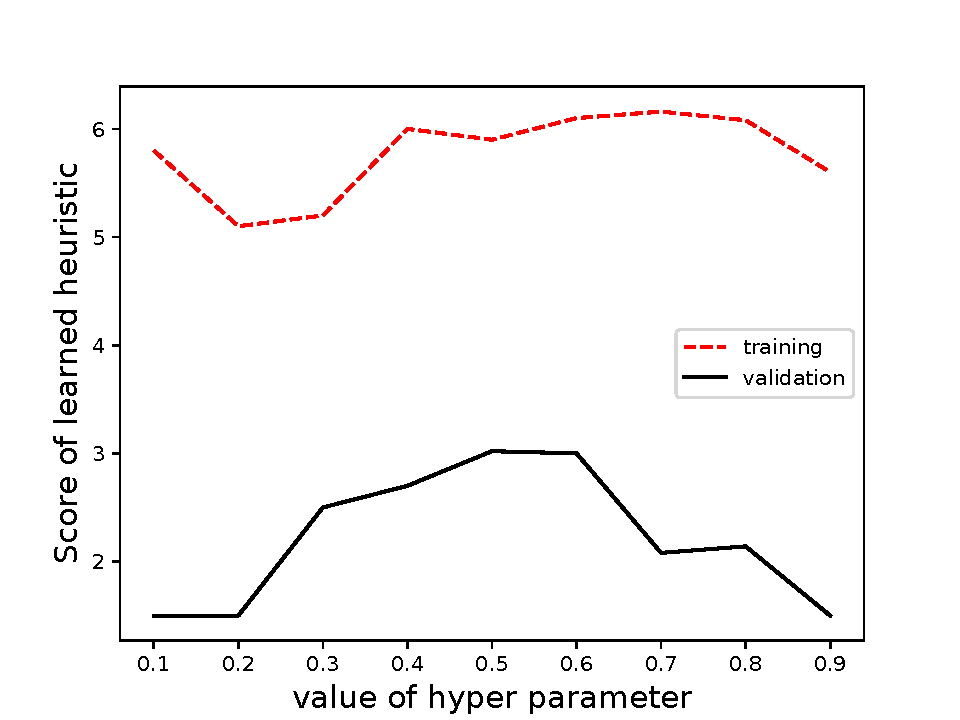
\includegraphics[width=6.3cm]{Graphick/figures/ctx_gamma.pdf}
	\caption{Object-sensitivity heuristic}
	\end{subfigure}
~\columnbreak

	\begin{subfigure}[t]{1.\columnwidth}
	\centering	
	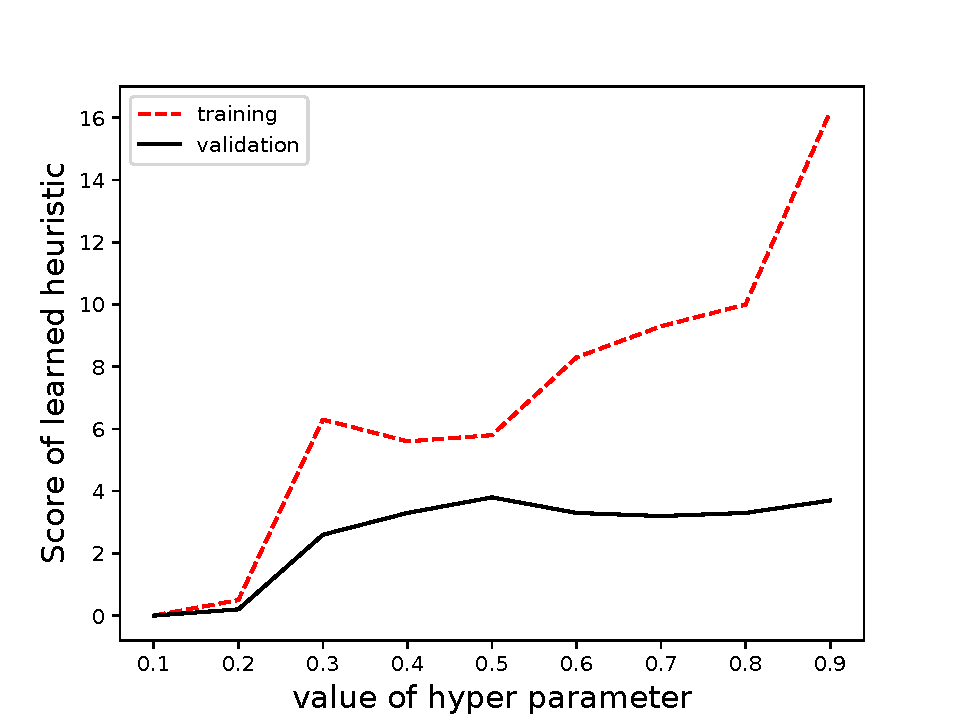
\includegraphics[width=6.3cm]{Graphick/figures/heap_gamma.pdf}
	\caption{Heap abstraction heuristic}
	\end{subfigure}
	\end{multicols}
	\caption{How score of learned heuristic changes over the value of $\hyper$.}
	\label{fig:gamma}
\end{figure}


\myparagraph{Choosing Hyper-Parameter $\hyper$}\label{sec:hyper_param}

Through our evaluation, we observed that the value of the hyper-parameter $\hyper$ plays an important role in the performance of the learned heuristic.
Figure~\ref{fig:gamma} depicts how performance of learned heuristics changes over the values of  $\hyper$.
The X-axis presents the value of $\hyper$ set to learn each heuristic, and
the Y-axis presents scores that we measured for performance of each heuristic $\heuristic_{\hyper}$ according to
${\sum_{P\in\vec{P}}\projproved(F_P(\heuristic_{\hyper}(G)))}\over{\sum_{P\in\vec{P}}
  \projcost(F_P(\heuristic_{\hyper}(G)))}$ where $\projcost$ denotes analysis time.
This score function presents the number of queries proved per second; thereby, more precise and scalable the analysis,
higher the score.
The red dotted and black solid lines present how the scores change over
the training programs $\vec{P}$ %(e.g., $\vec{P}$ = \{{\tt luindex,lusearch,antlr}\})
and the validation program, respectively.
For the training programs, the score of the learned heuristic increases as the higher $\hyper$ is given
because the heuristic becomes more fitted to the training programs.\footnote{It learned a bit bad heuristic when $\hyper$ is 0.9 in
  object-sensitivity heuristic because it is
difficult to generate specific features that satisfy such high precision
constraints; it eventually generates a general feature that include lots
of nodes.}
In our evaluation, both learned heuristics, however, perform the best on the validation program when $\hyper$ is 0.5;
thus, \OurCtx~in Table~\ref{tbl:contextAbstraction} and Table~\ref{tbl:heapAbstraction} corresponds to $\heuristic_{0.5}$.


%This occurs because the learned heuristics become overfitted to the training programs as the value of $\hyper$ increases;
%thus, simply increasing $\hyper$ is not an answer to achieve the best performance on validation and testing programs.







%\subsection{Learning Adequacy}

%\subsection{Insights from Generated Features}
\subsection{Learned Insights}

The learning algorithm generated 197 features in total for the object-sensitivity heuristic (68 features for 2-object-sensitivity, 29 for 2-type-sensitivity, and 100 features for 1-type-sensitivity). It generated 96 features for the heap abstraction heuristic.

\newcolumntype{P}[1]{>{\centering\arraybackslash}p{#1}}
\newcolumntype{M}[1]{>{\centering\arraybackslash}m{#1}}
\begin{figure}
\centering
\scriptsize
\setlength\extrarowheight{-1pt}
\begin{tabular}{|c|c|c| c | c | c |}
\toprule
\multicolumn{1}{|c}{}
                                                &                        & \multicolumn{1}{c|}{\textsf{Top 5 Features}} & \textsf{portion}
&\textsf{score} &
\multicolumn{1}{c|}{
\makecell{\textsf{Concretization}\\(Top 1)}
} \\ \midrule

\multirow{30}{*}{\rotatebox[origin=c]{90}{Object-Sensitivity Heuristic}}
& \multirow{10}{*}{\rotatebox[origin=c]{90}{1type}} &
\multirow{2}{*}{
\resizebox{0.40\columnwidth}{!}{
	\begin{tikzpicture}
	\node [block3,fill = gray] (n2) {{\tt\small [0,$\infty$],[61,$\infty$]}};
	\node [block3,right = 0.8cm of n2] (n3) {{\tt\small [46,$\infty$],[0,$\infty$]}};
	\path [line] (n2) -> (n3);
	\end{tikzpicture}
}
}
&\multirow{2}{*}{47\%} &\multirow{2}{*}{0.57}
                                        & \multirow{10}{*}{
		\resizebox{0.15\columnwidth}{!}{
			\begin{tikzpicture}
			\node [shape=circle,fill = gray,draw=black] (n1) {{\tt
                            n2}};
			\node [shape=circle,fill = gray,draw=black,left = 0.3cm
                        of n1] (n1left) {{\tt n1}};
			\node [shape=circle,fill = gray,draw=black,right = 0.3cm
                        of n1] (n1right) {{\tt n3}};
			\node [None,above = 0.7cm
                        of n1] (aboven1) {};
			\node [None,above = 0.7cm
                        of n1left] (aboven2) {};
			\node [None,above = 0.7cm
                        of n1right] (aboven3) {};
			\node [shape=circle,draw=black,below = 0.9cm
                        of n1] (n2) {{\tt n4}};
			\node [None,above left = 0.6 and 0.1cm
                        of n1] (n4) {};
			\node [None,right = 0.7cm
                        of n4] (n5) {};
			\node [None,above left = 0.7 and 0.5cm
                        of n2] (d1) {};
			\node [None, right = -0.1
                        of d1] (d2) {};
			\node [None, right = -0.1
                        of d2] (d3) {};
			\node [None, right = -0.1
                        of d3] (d4) {};
			\node [None, right = -0.1
                        of d4] (d5) {};
			\node [None, right = -0.1
                        of d5] (d6) {};
			\node [None, right = -0.1
                        of d6] (d7) {};
			\node [None, right = -0.1
                        of d7] (d8) {};
			\node [None, right = -0.1
                        of d8] (d9) {};
			\node [None, right = -0.1
                        of d9] (d10) {};
			\node [None, right = -0.1
                        of d10] (d11) {};
			\node [None, right = -0.1
                        of d11] (d12) {};
			\node [None, right = -0.1
                        of d12] (d13) {};		
			\path [line] (aboven1) -- (n1);
			\path [line] (aboven2) -- (n1left);
			\path [line] (aboven3) -- (n1right);
			\path [line] (n1left) -- (n2);
			\path [line] (n1right) -- (n2);
			\path [line] (n1) -- (n2);
			\path [line] (d1) -- (n2);
			\path [line] (d2) -- (n2);
			\path [line] (d3) -- (n2);
			\path [line] (d4) -- (n2);
			\path [line] (d5) -- (n2);
			\path [line] (d6) -- (n2);
			\path [line] (d7) -- (n2);
			\path [line] (d8) -- (n2);
			\path [line] (d9) -- (n2);
			\path [line] (d10) -- (n2);
			\path [line] (d11) -- (n2);
			\path [line] (d12) -- (n2);
			\path [line] (d13) -- (n2);
			\end{tikzpicture}
		}
}
                   \\
&&\multicolumn{1}{c|}{}&\multicolumn{1}{c|}{}  &\multicolumn{1}{c|}{}&\multicolumn{1}{c|}{}

\\
                                                &                        &
\multirow{2}{*}{
\resizebox{0.40\columnwidth}{!}{
	\begin{tikzpicture}
	\node [block3,fill = gray] (n2) {{\tt\small [0,$\infty$],[0,$\infty$]}};
	\node [block4,right = 0.8cm of n2] (n3) {{\tt\small [0,$\infty$],[117,$\infty$]}};
	\path [line] (n2) -> (n3);
	\end{tikzpicture}
}}
& \multirow{2}{*}{36\%} &\multirow{2}{*}{0.63}                                        &                                     \\
&&\multicolumn{1}{c|}{}&\multicolumn{1}{c|}{}  &\multicolumn{1}{c|}{}&\multicolumn{1}{c|}{}
\\
                                                &                        &
\multirow{2}{*}{
\resizebox{0.41\columnwidth}{!}{
	\begin{tikzpicture}
	\node [block4] (n2) {{\tt\small [0,$\infty$],[100,$\infty$]}};
	\node [block3,fill = gray,right = 0.8cm of n2] (n3) {{\tt\small [0,$\infty$],[29,$\infty$]}};
	\path [line] (n2) -> (n3);
	\end{tikzpicture}
}}
& \multirow{2}{*}{35\%} & \multirow{2}{*}{0.55}                                      &                                     \\
&&\multicolumn{1}{c|}{}&\multicolumn{1}{c|}{}  &\multicolumn{1}{c|}{}&\multicolumn{1}{c|}{}
\\
                                                &                        &
\multirow{2}{*}{
\resizebox{0.50\columnwidth}{!}{
	\begin{tikzpicture}
	\node [block4] (n2) {{\tt\small [0,$\infty$],[100,$\infty$]}};
	\node [block3,fill = gray,right = 0.3cm of n2] (n3) {{\tt\small [0,$\infty$],[0,$\infty$]}};
	\node [block4,right = 0.3cm of n3] (n4) {{\tt\small [0,$\infty$],[36,43]}};
	\path [line] (n2) -> (n3);
	\path [line] (n3) -> (n4);
	\end{tikzpicture}
}}
& \multirow{2}{*}{29\%} & \multirow{2}{*}{0.71}                                          &                                     \\
&&\multicolumn{1}{c|}{}&\multicolumn{1}{c|}{}  &\multicolumn{1}{c|}{}&\multicolumn{1}{c|}{}
\\


                                                &                        &
\multirow{2}{*}{
\resizebox{0.5\columnwidth}{!}{
	\begin{tikzpicture}
	\node [block4] (n2) {{\tt\small [0,$\infty$],[109,$\infty$]}};
	\node [block3,fill = gray,right = 0.3cm of n2] (n3) {{\tt\small [0,$\infty$],[0,$\infty$]}};
	\node [block4,right = 0.3cm of n3] (n4) {{\tt\small [171,$\infty$],[0,$\infty$]}};
	\path [line] (n2) -> (n3);
	\path [line] (n3) -> (n4);
	\end{tikzpicture}
}}
&\multirow{2}{*}{25\%}&\multirow{2}{*}{0.57}                                       &                                     \\
&&\multicolumn{1}{c|}{}&\multicolumn{1}{c|}{}  &\multicolumn{1}{c|}{}&\multicolumn{1}{c|}{}\\





\cline{2-6}
                                                & \multirow{10}{*}{\rotatebox[origin=c]{90}{2type}} &
\multirow{2}{*}{
\resizebox{0.40\columnwidth}{!}{
	\begin{tikzpicture}
	\node [block3] (n2) {{\tt\small [0,$\infty$],[36,39]}};
	\node [None ,above = 0.0cm of n2] (None) {};
	\node [block4 ,fill = gray,right = 0.8cm of n2] (n3) {{\tt\small [0,$\infty$],[73,75]}};
	\path [line] (n2) -> (n3);
	\end{tikzpicture}
}}
& \multirow{2}{*}{9\%}&\multirow{2}{*}{0.66}
                                                                                         & \multirow{10}{*}{
		\resizebox{0.15\columnwidth}{!}{
			\begin{tikzpicture}
			\node [shape=circle,fill = gray,draw=black] (n1) {{\tt
                            n2}};
			\node [shape=circle,draw=black,above = 0.5cm
                        of n1] (n0) {{\tt n1}};
			\node [None,below = 0.3cm
                        of n2] (bot) {};
			\node [None,right = 0.3cm
                        of n1] (n3) {};
			\node [None,above left = 0.4 and 0.5cm
                        of n0] (1d1) {};
			\node [None, right = -0.1
                        of 1d1] (1d2) {};
			\node [None, right = -0.1
                        of 1d2] (1d3) {};
			\node [None, right = -0.1
                        of 1d3] (1d4) {};
			\node [None, right = -0.1
                        of 1d4] (1d5) {};
			\node [None, right = -0.1
                        of 1d5] (1d6) {};
			\node [None, right = -0.1
                        of 1d6] (1d7) {};
			\node [None, right = -0.1
                        of 1d7] (1d8) {};
			\node [None, right = -0.1
                        of 1d8] (1d9) {};
			\node [None, right = -0.1
                        of 1d9] (1d10) {};
			\node [None, right = -0.1
                        of 1d10] (1d11) {};
			\node [None, right = -0.1
                        of 1d11] (1d12) {};
			\node [None, right = -0.1
                        of 1d12] (1d13) {};
			\node [None,below left = 0.3 and 0.7cm
                        of n0] (1e1) {};
			\node [None, right = -0.1
                        of 1e1] (1e2) {};
			\node [None, right = -0.1
                        of 1e2] (1e3) {};
			\node [None, right = -0.1
                        of 1e3] (1e4) {};
			\node [None, right = -0.1
                        of 1e4] (1e5) {};
			\node [None, right = -0.1
                        of 1e5] (1e6) {};
			\node [None, right = -0.1
                        of 1e6] (1e7) {};
			\node [None, right = -0.1
                        of 1e7] (1e8) {};
			\node [None, right = -0.1
                        of 1e8] (1e9) {};
			\node [None, right = -0.1
                        of 1e9] (1e10) {};
			\node [None, right = -0.1
                        of 1e10] (1e11) {};
			\node [None, right = -0.1
                        of 1e11] (1e12) {};
			\node [None, right = -0.1
                        of 1e12] (1e13) {};
			\node [None, right = -0.1
                        of 1e13] (1e14) {};
			\node [None, right = -0.1
                        of 1e14] (1e15) {};		
			\node [None,above left = 0.4 and 0.5cm
                        of n1] (d1) {};
			\node [None, right = -0.1
                        of d1] (d2) {};
			\node [None, right = -0.1
                        of d2] (d3) {};
			\node [None, right = -0.1
                        of d3] (d4) {};
			\node [None, right = -0.1
                        of d4] (d5) {};
			\node [None, right = -0.1
                        of d5] (d6) {};
			\node [None, right = -0.1
                        of d6] (d7) {};
			\node [None, right = -0.1
                        of d7] (d8) {};
			\node [None, right = -0.1
                        of d8] (d9) {};
			\node [None, right = -0.1
                        of d9] (d10) {};
			\node [None, right = -0.1
                        of d10] (d11) {};
			\node [None, right = -0.1
                        of d11] (d12) {};
			\node [None, right = -0.1
                        of d12] (d13) {};
			\node [None,below left = 0.5 and 0.7cm
                        of n1] (e1) {};
			\node [None, right = -0.1
                        of e1] (e2) {};
			\node [None, right = -0.1
                        of e2] (e3) {};
			\node [None, right = -0.1
                        of e3] (e4) {};
			\node [None, right = -0.1
                        of e4] (e5) {};
			\node [None, right = -0.1
                        of e5] (e6) {};
			\node [None, right = -0.1
                        of e6] (e7) {};
			\node [None, right = -0.1
                        of e7] (e8) {};
			\node [None, right = -0.1
                        of e8] (e9) {};
			\node [None, right = -0.1
                        of e9] (e10) {};
			\node [None, right = -0.1
                        of e10] (e11) {};
			\node [None, right = -0.1
                        of e11] (e12) {};
			\node [None, right = -0.1
                        of e12] (e13) {};
			\node [None, right = -0.1
                        of e13] (e14) {};
			\node [None, right = -0.1
                        of e14] (e15) {};			
%			\path [line] (n0) -- (1e1);
			\path [line] (n0) -- (1e2);
			\path [line] (n0) -- (1e3);
			\path [line] (n0) -- (1e4);
			\path [line] (n0) -- (1e5);
			\path [line] (n0) -- (1e6);
			\path [line] (n0) -- (1e7);
			\path [line] (n0) -- (1e8);
			\path [line] (n0) -- (1e9);
			\path [line] (n0) -- (1e10);
			\path [line] (n0) -- (1e11);
			\path [line] (n0) -- (1e12);
			\path [line] (n0) -- (1e13);
			\path [line] (n0) -- (1e14);
%			\path [line] (n0) -- (1e15);
			\path [line] (n0) -- (n1);
%			\path [line] (n1) -- (e1);
			\path [line] (n1) -- (e2);
			\path [line] (n1) -- (e3);
			\path [line] (n1) -- (e4);
			\path [line] (n1) -- (e5);
			\path [line] (n1) -- (e6);
			\path [line] (n1) -- (e7);
			\path [line] (n1) -- (e8);
			\path [line] (n1) -- (e9);
			\path [line] (n1) -- (e10);
			\path [line] (n1) -- (e11);
			\path [line] (n1) -- (e12);
			\path [line] (n1) -- (e13);
			\path [line] (n1) -- (e14);
%			\path [line] (n1) -- (e15);
			\end{tikzpicture}
		}
}                   \\
&&\multicolumn{1}{c|}{}&\multicolumn{1}{c|}{}  &\multicolumn{1}{c|}{}&\multicolumn{1}{c|}{}
\\
                                                &                        &
\multirow{2}{*}{
\resizebox{0.18\columnwidth}{!}{
	\begin{tikzpicture}
	\node [block4,fill = gray] (n2) {{\tt\small [105,155],[0,$\infty$]}};
	\end{tikzpicture}
}}
&\multirow{2}{*}{9\%}&\multirow{2}{*}{1} 
&                                     \\
&&\multicolumn{1}{c|}{}&\multicolumn{1}{c|}{}  &\multicolumn{1}{c|}{}&\multicolumn{1}{c|}{}
\\
                                                &                        &
\multirow{2}{*}{
\resizebox{0.5\columnwidth}{!}{
	\begin{tikzpicture}
	\node [block3] (n2) {{\tt\small [0,$\infty$],[0,61]}};
	\node [block4,fill = gray,right = 0.3cm of n2] (n3) {{\tt\small [60,76],[0,61]}};
	\node [block3,right = 0.3cm of n3] (n4) {{\tt\small [0,22],[0,$\infty$]}};
	\path [line] (n2) -> (n3);
	\path [line] (n3) -> (n4);
	\end{tikzpicture}
}}
& \multirow{2}{*}{9\%} &\multirow{2}{*}{0.5}                                          &                                     \\
&&\multicolumn{1}{c|}{}&\multicolumn{1}{c|}{}  &\multicolumn{1}{c|}{}&\multicolumn{1}{c|}{}
\\
                                                &                        &
\multirow{2}{*}{
\resizebox{0.5\columnwidth}{!}{
	\begin{tikzpicture}
	\node [block3] (n2) {{\tt\small [0,$\infty$],[29,61]}};
	\node [block4,fill = gray,right = 0.3cm of n2] (n3) {{\tt\small [171,228],[0,$\infty$]}};
	\node [block3,right = 0.3cm of n3] (n4) {{\tt\small [0,46],[0,$\infty$]}};
	\path [line] (n2) -> (n3);
	\path [line] (n3) -> (n4);
	\end{tikzpicture}
}}
&\multirow{2}{*}{4\%} &\multirow{2}{*}{1}                                       &                                     \\
&&\multicolumn{1}{c|}{}&\multicolumn{1}{c|}{}  &\multicolumn{1}{c|}{}&\multicolumn{1}{c|}{}
\\
                                                &                        &
\multirow{2}{*}{
\resizebox{0.18\columnwidth}{!}{
	\begin{tikzpicture}
	\node [block3,fill = gray] (n2) {{\tt\small [84,91],[0,$\infty$]}};
	\end{tikzpicture}
}}
& \multirow{2}{*}{4\%} & \multirow{2}{*}{0.5}                                      &                                     \\
&&\multicolumn{1}{c|}{}&\multicolumn{1}{c|}{}  &\multicolumn{1}{c|}{}&\multicolumn{1}{c|}{}
\\
\cline{2-6}
 & \multirow{10}{*}{\rotatebox[origin=c]{90}{2obj}}  &
\multirow{2}{*}{
\resizebox{0.17\columnwidth}{!}{
	\begin{tikzpicture}
	\node [block3,fill = gray] (n2) {{\tt\small [0,$\infty$],[53,61]}};
	\node [None ,above = 0.0cm of n2] (None) {};
	\end{tikzpicture}
}}
& \multirow{2}{*}{9\%} & \multirow{2}{*}{0.53}
& \multirow{10}{*}{
\resizebox{0.15\columnwidth}{!}{
			\begin{tikzpicture}
			\node [None] (n1) {};
			\node [shape=circle,fill=gray,draw=black,below = 0.9cm
                        of n1] (n2) {{\tt n1}};
			\node [None,right = 0.3cm
                        of n1] (n3) {};
			\node [None,above left = 0.7 and 0.5cm
                        of n2] (d1) {};
			\node [None, right = -0.1
                        of d1] (d2) {};
			\node [None, right = -0.1
                        of d2] (d3) {};
			\node [None, right = -0.1
                        of d3] (d4) {};
			\node [None, right = -0.1
                        of d4] (d5) {};
			\node [None, right = -0.1
                        of d5] (d6) {};
			\node [None, right = -0.1
                        of d6] (d7) {};
			\node [None, right = -0.1
                        of d7] (d8) {};
			\node [None, right = -0.1
                        of d8] (d9) {};
			\node [None, right = -0.1
                        of d9] (d10) {};
			\node [None, right = -0.1
                        of d10] (d11) {};
			\node [None, right = -0.1
                        of d11] (d12) {};
			\node [None, right = -0.1
                        of d12] (d13) {};
			\node [None,below left = 0.9 and 0.7cm
                        of n2] (e1) {};
			\node [None, right = -0.1
                        of e1] (e2) {};
			\node [None, right = -0.1
                        of e2] (e3) {};
			\node [None, right = -0.1
                        of e3] (e4) {};
			\node [None, right = -0.1
                        of e4] (e5) {};
			\node [None, right = -0.1
                        of e5] (e6) {};
			\node [None, right = -0.1
                        of e6] (e7) {};
			\node [None, right = -0.1
                        of e7] (e8) {};
			\node [None, right = -0.1
                        of e8] (e9) {};
			\node [None, right = -0.1
                        of e9] (e10) {};
			\node [None, right = -0.1
                        of e10] (e11) {};
			\node [None, right = -0.1
                        of e11] (e12) {};
			\node [None, right = -0.1
                        of e12] (e13) {};
			\node [None, right = -0.1
                        of e13] (e14) {};
			\node [None, right = -0.1
                        of e14] (e15) {};			
			\path [line] (n1) -- (n2);
%			\path [line] (n2) -- (e1);
			\path [line] (n2) -- (e2);
			\path [line] (n2) -- (e3);
			\path [line] (n2) -- (e4);
			\path [line] (n2) -- (e5);
			\path [line] (n2) -- (e6);
			\path [line] (n2) -- (e7);
			\path [line] (n2) -- (e8);
			\path [line] (n2) -- (e9);
			\path [line] (n2) -- (e10);
			\path [line] (n2) -- (e11);
			\path [line] (n2) -- (e12);
			\path [line] (n2) -- (e13);
			\path [line] (n2) -- (e14);
%			\path [line] (n2) -- (e15);
			\end{tikzpicture}
		}
}                   \\
&&\multicolumn{1}{c|}{}&\multicolumn{1}{c|}{}  &\multicolumn{1}{c|}{}&\multicolumn{1}{c|}{}
\\
                                                &
                                                                        &
\multirow{2}{*}{
\resizebox{0.17\columnwidth}{!}{
\begin{tikzpicture}
\node [block3,fill = gray] (n2) {{\tt\small [0,$\infty$],[24,25]}};
\end{tikzpicture}
}}
&\multirow{2}{*}{6\%} &\multirow{2}{*}{0.53}                                       &                                     \\
&&\multicolumn{1}{c|}{}&\multicolumn{1}{c|}{}  &\multicolumn{1}{c|}{}&\multicolumn{1}{c|}{}
\\
                                                &                        &
\multirow{2}{*}{\resizebox{0.5\columnwidth}{!}{
	\begin{tikzpicture}
	\node [block4,fill = gray] (n2) {{\tt\small [0,$\infty$],[0,7]}};
	\node [block3,right = 0.3cm of n2] (n3) {{\tt\small [9,11],[0,$\infty$]}};
	\node [block3,right = 0.3cm of n3] (n4) {{\tt\small [76,$\infty$],[0,$\infty$]}};
	\path [line] (n2) -> (n3);
	\path [line] (n3) -> (n4);
	\end{tikzpicture}
}}
&\multirow{2}{*}{2\%}&\multirow{2}{*}{0.82}                                        & \\
&&\multicolumn{1}{c|}{}&\multicolumn{1}{c|}{}  &\multicolumn{1}{c|}{}&\multicolumn{1}{c|}{}
\\

                                                &                        &
\multirow{2}{*}{\resizebox{0.5\columnwidth}{!}{
	\begin{tikzpicture}
	\node [block4] (n2) {{\tt\small [0,$\infty$],[43,$\infty$]}};
	\node [block3,fill = gray,right = 0.3cm of n2] (n3) {{\tt\small [0,$\infty$],[0,14]}};
	\node [block3,right = 0.3cm of n3] (n4) {{\tt\small [22,24],[0,$\infty$]}};
	\path [line] (n2) -> (n3);
	\path [line] (n3) -> (n4);
	\end{tikzpicture}
}}
&\multirow{2}{*}{1\%}&\multirow{2}{*}{0.63}                                        &                                     \\
&&\multicolumn{1}{c|}{}&\multicolumn{1}{c|}{}  &\multicolumn{1}{c|}{}&\multicolumn{1}{c|}{}
\\
                                                &
                                                                        &
\multirow{2}{*}{\resizebox{0.5\columnwidth}{!}{
	\begin{tikzpicture}
	\node [block4] (n2) {{\tt\small [0,$\infty$],[145,147]}};
	\node [block3,fill = gray,right = 0.3cm of n2] (n3) {{\tt\small [0,$\infty$],[0,$\infty$]}};
	\node [block3,right = 0.3cm of n3] (n4) {{\tt\small [0,46],[0,$\infty$]}};
	\path [line] (n2) -> (n3);
	\path [line] (n3) -> (n4);
	\end{tikzpicture}
}}                                                                                &\multirow{2}{*}{1\%}&\multirow{2}{*}{0.69}&                                     \\
&&\multicolumn{1}{c|}{}&\multicolumn{1}{c|}{}  &\multicolumn{1}{c|}{}&\multicolumn{1}{c|}{}
\\

%                                                &                        &
%\resizebox{0.45\columnwidth}{!}{
%	\begin{tikzpicture}
%	\node [block3,fill = gray] (n2) {{\tt\small [0,$\infty$],[0,3]}};
%	\node [block4,right = 0.8cm of n2] (n3) {{\tt\small [22,33],[0,$\infty$]}};
%	\path [line] (n2) -> (n3);
%	\end{tikzpicture}
%}                                       &                                     \\
 \midrule\midrule
\multicolumn{2}{|c|}{\multirow{10}{*}{
		\rotatebox[origin=c]{90}{\makecell{Heap Abstraction\\Heuristic}}}}        &
\multirow{2}{*}{\resizebox{0.5\columnwidth}{!}{
	\begin{tikzpicture}
	\node [block3,fill = gray] (n2) {{\tt\small [0,$\infty$],[0,3]}};
	\node [block4,right = 0.3cm of n2] (n3) {{\tt\small [48,$\infty$],[0,$\infty$]}};
	\node [block4,right = 0.3cm of n3] (n4) {{\tt\small [0,$\infty$],[140,$\infty$]}};
	\path [line] (n2) -> (n3);
	\path [line] (n3) -> (n4);
	\end{tikzpicture}
}}
& \multirow{2}{*}{35\%} &\multirow{2}{*}{0.61} 

& \multirow{10}{*}{
		\resizebox{0.15\columnwidth}{!}{
			\begin{tikzpicture}
			\node [shape=circle,fill = gray,draw=black] (n1) {{\tt
                            n1}};
			\node [shape=circle,draw=black,below = 0.6cm
                        of n1] (n2) {{\tt n2}};
			\node [shape=circle,draw=black,below = 0.6cm
                        of n2] (n4) {{\tt n3}};
			\node [None,right = 0.3cm
                        of n1] (n3) {};
			\node [None,above left = 0.5 and 0.5cm
                        of n2] (d1) {};
			\node [None, right = -0.1
                        of d1] (d2) {};
			\node [None, right = -0.1
                        of d2] (d3) {};
			\node [None, right = -0.1
                        of d3] (d4) {};
			\node [None, right = -0.1
                        of d4] (d5) {};
			\node [None, right = -0.1
                        of d5] (d6) {};
			\node [None, right = -0.1
                        of d6] (d7) {};
			\node [None, right = -0.1
                        of d7] (d8) {};
			\node [None, right = -0.1
                        of d8] (d9) {};
			\node [None, right = -0.1
                        of d9] (d10) {};
			\node [None, right = -0.1
                        of d10] (d11) {};
			\node [None, right = -0.1
                        of d11] (d12) {};
			\node [None, right = -0.1
                        of d12] (d13) {};
			\node [None,below left = 0.4 and 0.7cm
                        of n2] (e1) {};
			\node [None, right = -0.1
                        of e1] (e2) {};
			\node [None, right = -0.1
                        of e2] (e3) {};
			\node [None, right = -0.1
                        of e3] (e4) {};
			\node [None, right = -0.1
                        of e4] (e5) {};
			\node [None, right = -0.1
                        of e5] (e6) {};
			\node [None, right = -0.1
                        of e6] (e7) {};
			\node [None, right = -0.1
                        of e7] (e8) {};
			\node [None, right = -0.1
                        of e8] (e9) {};
			\node [None, right = -0.1
                        of e9] (e10) {};
			\node [None, right = -0.1
                        of e10] (e11) {};
			\node [None, right = -0.1
                        of e11] (e12) {};
			\node [None, right = -0.1
                        of e12] (e13) {};
			\node [None, right = -0.1
                        of e13] (e14) {};
			\node [None, right = -0.1
                        of e14] (e15) {};	
			\node [None,above left = 0.3 and 0.5cm
                        of n4] (1d1) {};
			\node [None, right = -0.1
                        of 1d1] (1d2) {};
			\node [None, right = -0.1
                        of 1d2] (1d3) {};
			\node [None, right = -0.1
                        of 1d3] (1d4) {};
			\node [None, right = -0.1
                        of 1d4] (1d5) {};
			\node [None, right = -0.1
                        of 1d5] (1d6) {};
			\node [None, right = -0.1
                        of 1d6] (1d7) {};
			\node [None, right = -0.1
                        of 1d7] (1d8) {};
			\node [None, right = -0.1
                        of 1d8] (1d9) {};
			\node [None, right = -0.1
                        of 1d9] (1d10) {};
			\node [None, right = -0.1
                        of 1d10] (1d11) {};
			\node [None, right = -0.1
                        of 1d11] (1d12) {};
			\node [None, right = -0.1
                        of 1d12] (1d13) {};
			\node [None,below left = 0.5 and 0.7cm
                        of n4] (1e1) {};
			\node [None, right = -0.1
                        of 1e1] (1e2) {};
			\node [None, right = -0.1
                        of 1e2] (1e3) {};
			\node [None, right = -0.1
                        of 1e3] (1e4) {};
			\node [None, right = -0.1
                        of 1e4] (1e5) {};
			\node [None, right = -0.1
                        of 1e5] (1e6) {};
			\node [None, right = -0.1
                        of 1e6] (1e7) {};
			\node [None, right = -0.1
                        of 1e7] (1e8) {};
			\node [None, right = -0.1
                        of 1e8] (1e9) {};
			\node [None, right = -0.1
                        of 1e9] (1e10) {};
			\node [None, right = -0.1
                        of 1e10] (1e11) {};
			\node [None, right = -0.1
                        of 1e11] (1e12) {};
			\node [None, right = -0.1
                        of 1e12] (1e13) {};
			\node [None, right = -0.1
                        of 1e13] (1e14) {};
			\node [None, right = -0.1
                        of 1e14] (1e15) {};				
			\path [line] (n1) -- (n2);
			\path [line] (n1) -- (n3);
			\path [line] (d1) -- (n2);
			\path [line] (d2) -- (n2);
			\path [line] (d3) -- (n2);
			\path [line] (d4) -- (n2);
			\path [line] (d5) -- (n2);
			\path [line] (d6) -- (n2);
			\path [line] (d7) -- (n2);
			\path [line] (d8) -- (n2);
			\path [line] (d9) -- (n2);
			\path [line] (d10) -- (n2);
			\path [line] (d11) -- (n2);
			\path [line] (d12) -- (n2);
			\path [line] (d13) -- (n2);
%			\path [line] (n2) -- (e1);
			\path [line] (n2) -- (e2);
			\path [line] (n2) -- (e3);
			\path [line] (n2) -- (e4);
			\path [line] (n2) -- (e5);
			\path [line] (n2) -- (e6);
			\path [line] (n2) -- (e7);
			\path [line] (n2) -- (e8);
			\path [line] (n2) -- (e9);
			\path [line] (n2) -- (e10);
			\path [line] (n2) -- (e11);
			\path [line] (n2) -- (e12);
			\path [line] (n2) -- (e13);
			\path [line] (n2) -- (e14);
%			\path [line] (n2) -- (e15);
			\path [line] (n2) -- (n4);
			\path [line] (1d1) -- (n4);
			\path [line] (1d2) -- (n4);
			\path [line] (1d3) -- (n4);
			\path [line] (1d4) -- (n4);
			\path [line] (1d5) -- (n4);
			\path [line] (1d6) -- (n4);
			\path [line] (1d7) -- (n4);
			\path [line] (1d8) -- (n4);
			\path [line] (1d9) -- (n4);
			\path [line] (1d10) -- (n4);
			\path [line] (1d11) -- (n4);
			\path [line] (1d12) -- (n4);
			\path [line] (1d13) -- (n4);
%			\path [line] (n4) -- (1e1);
			\path [line] (n4) -- (1e2);
			\path [line] (n4) -- (1e3);
			\path [line] (n4) -- (1e4);
			\path [line] (n4) -- (1e5);
			\path [line] (n4) -- (1e6);
			\path [line] (n4) -- (1e7);
			\path [line] (n4) -- (1e8);
			\path [line] (n4) -- (1e9);
			\path [line] (n4) -- (1e10);
			\path [line] (n4) -- (1e11);
			\path [line] (n4) -- (1e12);
			\path [line] (n4) -- (1e13);
			\path [line] (n4) -- (1e14);
%			\path [line] (n4) -- (1e15);
			\end{tikzpicture}
		}
}\\
\multicolumn{1}{|c}{}&\multicolumn{1}{c|}{}&\multicolumn{1}{c|}{}&\multicolumn{1}{c|}{}  &\multicolumn{1}{c|}{}&\multicolumn{1}{c|}{}
\\
\multicolumn{2}{|l|}{}                                                   &
\multirow{2}{*}{\resizebox{0.5\columnwidth}{!}{
	\begin{tikzpicture}
	\node [block3,fill = gray] (n2) {{\tt\small [0,12],[0,3]}};
	\node [block4,right = 0.3cm of n2] (n3) {{\tt\small [0,97],[0,$\infty$]}};
	\node [block4,right = 0.3cm of n3] (n4) {{\tt\small [0,$\infty$],[140,$\infty$]}};
	\path [line] (n2) -> (n3);
	\path [line] (n3) -> (n4);
	\end{tikzpicture}
}}
&\multirow{2}{*}{33\%}
&\multirow{2}{*}{0.53}                                      &                                     \\
\multicolumn{1}{|c}{}&\multicolumn{1}{c|}{}&\multicolumn{1}{c|}{}&\multicolumn{1}{c|}{}  &\multicolumn{1}{c|}{}&\multicolumn{1}{c|}{}
\\
\multicolumn{2}{|l|}{}                                                   &
\multirow{2}{*}{\resizebox{0.40\columnwidth}{!}{
	\begin{tikzpicture}
	\node [block4,fill = gray] (n3) {{\tt\small [38,$\infty$],[0,62]}};
	\node [block4,right = 0.8cm of n3] (n4) {{\tt\small [0,$\infty$],[236,$\infty$]}};
	\path [line] (n3) -> (n4);
	\end{tikzpicture}
}}
& \multirow{2}{*}{27\%} &\multirow{2}{*}{0.59}                                        &                                     \\
\multicolumn{1}{|c}{}&\multicolumn{1}{c|}{}&\multicolumn{1}{c|}{}&\multicolumn{1}{c|}{}  &\multicolumn{1}{c|}{}&\multicolumn{1}{c|}{}
\\
\multicolumn{2}{|l|}{}                                                   &
\multirow{2}{*}{\resizebox{0.40\columnwidth}{!}{
	\begin{tikzpicture}
	\node [block4,fill = gray] (n3) {{\tt\small [0,48],[0,62]}};
	\node [block4,right = 0.8cm of n3] (n4) {{\tt\small [72,84],[0,$\infty$]}};
	\path [line] (n3) -> (n4);
	\end{tikzpicture}
}}
& \multirow{2}{*}{24\%} & \multirow{2}{*}{0.53} 
                                         &\\
\multicolumn{1}{|c}{}&\multicolumn{1}{c|}{}&\multicolumn{1}{c|}{}&\multicolumn{1}{c|}{}  &\multicolumn{1}{c|}{}&\multicolumn{1}{c|}{}
\\
\multicolumn{2}{|l|}{}                                                   &
\multirow{2}{*}{\resizebox{0.5\columnwidth}{!}{
	\begin{tikzpicture}
	\node [block3,fill = gray] (n2) {{\tt\small [0,24],[0,$\infty$]}};
	\node [block4,right = 0.3cm of n2] (n3) {{\tt\small [21,$\infty$],[140,$\infty$]}};
	\node [block4,right = 0.3cm of n3] (n4) {{\tt\small [0,97],[0,$\infty$]}};
	\path [line] (n2) -> (n3);
	\path [line] (n3) -> (n4);
	\end{tikzpicture}
}}
& \multirow{2}{*}{22\%} & \multirow{2}{*}{0.53} 
                                         &                                     \\
\multicolumn{1}{|c}{}&\multicolumn{1}{c|}{}&\multicolumn{1}{c|}{}&\multicolumn{1}{c|}{}  &\multicolumn{1}{c|}{}&\multicolumn{1}{c|}{}
\\
%\multicolumn{2}{|l|}{}                                                   &
%\resizebox{0.45\columnwidth}{!}{
%	\begin{tikzpicture}
%	\node [block3,fill = gray] (n2) {{\tt\small [0,48],[0,$\infty$]}};
%	\node [block4,right = 0.8cm of n2] (n3) {{\tt\small [72,84],[0,$\infty$]}};
%
%	\path [line] (n2) -> (n3);
%	\end{tikzpicture}
%}                                         &                                     \\
\bottomrule
\end{tabular}
\caption{Top-5 features learned by our technique, and concrete nodes implied by the top-1 feature.
%Gray colored abstract nodes in the features correspond to the target nodes and others are predecessors or successors.
%Gray colored nodes in the column \textsf{Concretization} are precision-critical nodes which are selected by the first features; 
%other nodes are predecessors or successors that make the gray colored nodes satisfy the features.
}
\label{fig:features}
\end{figure}



%%% Local Variables:
%%% mode: latex
%%% TeX-master: "paper"
%%% End:


\myparagraph{Top-5 Features}
Figure~\ref{fig:features} describes the most informative features generated by our technique for each abstraction degree and their concretization in the given graphs.
The second column \textsf{Top 5 Features}, in decreasing order of \textsf{portion}, presents top 5 features which have the greatest number of precision-critical nodes satisfying the features with scores above 0.5.
For example, the first feature in 1type contains 47\% nodes of the total precision-critical nodes which are to be applied 1-type-sensitivity,
and has a score of 0.57.
If a feature is too general (e.g., $(\epsilon, ([0,\infty],[0,\infty]), \epsilon)$), it is excluded even with a large portion (e.g., 100\%)
because its score is under 0.5.
Similarly, if a feature is too specific, it is also excluded because it includes a small number of precision-critical nodes even with a good score.
For the features, the gray colored abstract nodes correspond to the target one $\hat{n}$ in each feature
(e.g., $(\seq{\myhat{p}_0,\myhat{p}_1,\dots,\myhat{p}_q}, \myhat{n}, \seq{\myhat{s}_0,\myhat{s}_1,\dots,\myhat{s}_r}) \in \Feature$).
Other nodes are predecessors or successors of the target abstract nodes (e.g., $\myhat{p}_0$, $\myhat{s}_0$, and $\myhat{s}_1$).
For each feature, we show the number of satisfying nodes over the total precision-critical nodes in the given graphs (\textsf{portion}) and the scores (\textsf{score}).
The right most column, \textsf{Concretization}, illustrates the visualized concretization for each first feature in \textsf{Top 5 Features} column,
%in the real graphs over the training programs, where the gray colored nodes correspond to the target nodes of the first feature.
where the gray colored nodes correspond to the target abstract nodes of the first feature.
For space reasons, we draw each node to have at most 13 incoming and outgoing edges although it can have more than 13 edges.


\begin{table}[]
\setlength\extrarowheight{-1pt}
\caption{Performance of our manually-designed graph-based heap abstraction heuristic for FPG}
\label{tbl:principle}
\centering
\footnotesize
\begin{tabular}{@{}clrr | clrr@{}}
\toprule
benchmarks               & \multicolumn{1}{c}{} & \multicolumn{1}{c}{alarms} & \multicolumn{1}{c|}{time(s)} & benchmarks                & \multicolumn{1}{c}{} & \multicolumn{1}{c}{alarms} & \multicolumn{1}{c}{time(s)} \\ \midrule
\multirow{2}{*}{luindex} & \Principle              & 374                        & 29(+29)                         & \multirow{2}{*}{lusearch} & \Principle            & 388                        & 33(+31)                        \\
                         % & \OurHeap            & 358                        & 23                          &                           & \OurHeap              & 372                        & 21                          \\
                         & \AllocBased          & 358                        & 5,475                       &                           & \AllocBased          & -                          & $>$10,800        \\\midrule
\multirow{2}{*}{antlr}   & \Principle              & 478                        & 44(+47)                        & \multirow{2}{*}{pmd$_{m}$}      & \Principle            & 886                        & 83(+65)                          \\
                         % & \OurHeap            & 463                        & 49                          &                           & \OurHeap              & 871                        & 48                          \\
                         & \AllocBased          & 463                        & 5,241                       &                           & \AllocBased          & 871                        & 9,146                       \\\midrule
\multirow{2}{*}{fop}     & \Principle            & 391                        & 41(+46)                          & \multirow{2}{*}{xalan}    & \Principle            & 548                        & 841(+85)                         \\
                         % & \OurHeap              & 376                        & 30                          &                           & \OurHeap              & 539                        & 489                         \\
                         & \AllocBased          & -                          & $>$10,800        &                           & \AllocBased          & -                          & $>$10,800        \\ \bottomrule
\end{tabular}
\end{table}


\myparagraph{Insights}

The generated features during the learning process provide hints on designing analysis heuristics from the graphs.
For example, we investigated the features of the heap abstraction heuristic in Figure~\ref{fig:features} and found two commonalities in them.
First,  the features have the form of $(\epsilon,\hat{n}, \hat{\vec{s}})$ where $\hat{\vec{s}}$ is not $\epsilon$,
which implies that we should consider successors more than predecessors when designing heap abstraction heuristics from points-to graph.
The second commonality is that $\hat{\vec{s}}$ or $\hat{n}$ tends to include an abstract
node $\aNode$ that presents nodes with lots of outgoing edges, i.e., $\aNode =
(itv,[b,\infty])$ where the number $b$ is about $3\%$ of the total nodes in a graph of a training program.
From these observations, we manually designed a graph-based heap abstraction heuristic which
assigns allocation-site based heap abstraction to the target nodes
if at least $3\%$ of the total nodes in FPG belong to either the target node or its successor nodes
(i.e. $\heuristic = \seq{\{ (\epsilon,([0,\infty],[b',\infty]),\epsilon)
	,(\epsilon,\top,\seq{([0,\infty],[b',\infty])})
	,(\epsilon,\top,\seq{\top,([0,\infty],[b',\infty])})
	,\dots
	\}
}$ where $\top$ equals to the most general one $([0,\infty],[0,\infty])$ and $b'$ is 3\% of the total nodes in the given graph).
Otherwise, the heuristic assigns type-based heap abstraction to the others.
%where $\top$ equals to the most general abstract node $([0,\infty],[0,\infty])$, and $b$ equals to 3\% of the total nodes in the given graph).
Table~\ref{tbl:principle} demonstrates the performance of the manually-crafted heuristic.
In comparison to \AllocBased, it reduces about 99\% of analysis cost while producing only 2\% more alarms.
%Compared to the baseline heuristic~\AllocBased,



Intuitively, the nodes with lots of successors in FPG should be analyzed precisely because merging the objects with others would produce lots of spurious analysis results.
For example, if there exists an object with lots of field objects which we want to merge with another one with a few field objects,
it eventually produces lots of spurious results stating that the both heaps can have lots of field objects.
%Such insight is related with that of \Mahjong~which merges the two objects if they have the same types of successors because,
%statically, an object having lots of successors is hard to have exactly the same types of successors with other objects.
Such insight is related with that of \Mahjong~which merges the objects if their successors have the same type;
statistically, if an object has lots of successors, there hardly exist the other objects with exactly the same types of successors.
Surprisingly, it is easy to find such insight through the features generated by our technique.
Note that this insight is general as it is not dependent to Java programs.
For example, when analyzing a C program, it is a required task not to merge such heaps with others as it would produce lots of spurious results.

%\textcolor{black}{
%\myparagraph{Graphick vs Scaler}
%Interestingly, Figure~\ref{fig:features} shows that the insight learned statistically can differ from the logic-based insight
%through the difference between \OurCtx~and \Scaler~in deciding which nodes to analyze more precisely.
Interestingly, Figure~\ref{fig:features} also shows the difference between the statistically-learned insight behind \OurCtx~and the logical insight behind \Scaler~in deciding which nodes to analyze more precisely.
Based on the logical insight, \Scaler~relies heavily on the number of incoming edges
as that number in the object allocation graph indicates %{\color{red}{
how many contexts will be constructed in object sensitivity.%}}
~\ourtool, however, treats the number of neighbor nodes' outgoing edges more importantly, as shown in Figure 6.
Such differences result in the performance gap between the two object-sensitivity heuristics.
%which shows better performance in both precision and scalability than the logic-based insight.
%}

%\textcolor{red}{
\myparagraph{Generality of learned heuristic}
We found the learned heuristic for object sensitivity is general to the hybrid-context sensitivity~\cite{kastrinis2013hybrid}. Table~\ref{tbl:hybrid} presents the performance of the conventional 2-hybrid-context sensitivity (\twosobjH) and
2-hybrid-context sensitivity with the learned heuristic (\ourtool) used in Section~\ref{sec:comparescaler}.
%when using 6 DaCapo benchmark programs as testing programs.
The table shows that \ourtool~is also cost-effective compared to \twosobjH. For example, on a test program bloat,
\ourtool~produces only 22 more alarms while reducing about 90\% of analysis costs.
%}



\begin{table}[]
\setlength\extrarowheight{-1pt}
\caption{Performance comparison between conventional 2-hybrid-context-sensitivity (\twosobjH) and 2-hybrid-context-sensitivity with our learned heuristic for 2-object-sensitivity (\ourtool).}
\label{tbl:hybrid}
\centering\footnotesize
\begin{tabular}{@{}clrrrrrr@{}}
\toprule
                          & \multicolumn{1}{c}{} & \multicolumn{1}{c}{pmd$_m$} & \multicolumn{1}{c}{chart} & \multicolumn{1}{c}{eclipse} & \multicolumn{1}{c}{xalan} & \multicolumn{1}{c}{fop} & \multicolumn{1}{c}{bloat}  \\ \midrule
\multirow{2}{*}{\ourtool} & \#may-fail casts     & 220                      & 867                       & 2,880                        & 479                       & 1,408                    & 1,147                      \\
                          & analysis time (s)    & 45+(78)                  & 83(+76)                   & 1,426(+105)                  & 185(+57)                  & 245(+85)                & 215(+30)                  \\ \midrule
\multirow{2}{*}{\twosobjH}    & \#may-fail casts     & 220                      & 757                       & -                       & 447                          &  1,295                       & 1,125                          \\
                          & analysis time (s)    & 42                       & 195                       & >10,800                            & 428                          & 818                        & 2,238                           \\
%\midrule
%\multirow{2}{*}{\Insens}   & \#may-fail casts     & 679                      & 1,810                      & 4190                        & 1,182                      & 2,458                    & 1,924                      \\
%                          & analysis time (s)    & 23                       & 48                        & 91                          & 37                        & 53                      & 20                        \\
\bottomrule
\end{tabular}
\end{table}


\iffalse
\textcolor{red}{
%\myparagraph{Graphick vs Scaler}
Further, we could derive interesting differences between \ourtool~and Scaler in deciding which nodes to analyze more precisely.
Given an object allocation graph, Scaler relies heavily on the number of incoming edges
%into the target node in determining the context.
as the number of incoming edges reveals how each context will be constructed in object-sensitivity.
\ourtool, however, considers the number of neighbor nodes' outgoing edges more as shown in Figure 6,
which is statistically learned from training data.
%\ourtool~statistically found the consideration on the number of outgoing edges benefits the learned heuristic more.
%This results show that the logical insight (\Scaler) can be different from the statistical insight (\ourtool).
%\todored{more than just difference... any other insights..? why considering the outgoing more?}
}
\fi


%
%For example, Scaler is a heuristic that heavily reasons about the number of incoming edges' to target nodes for context decision. \ourtool, however, considers the number of neighbor nodes' outgoing edges more as shown in Figure 6. We will discuss this observation in the revised paper.
%}






%%% Local Variables:
%%% mode: latex
%%% TeX-master: "paper"
%%% End:
